%%%%%%%%%%%%%%%%%%%%%%%%%%%%%%%%%%%%%%%%%%%%%%%%%%%%%%%%%%%%%%%%%%
%%%%%%%%%%%%%%%%%%%%%%%%    TABLE 1     %%%%%%%%%%%%%%%%%%%%%%%%%%
%%%%%%%%%%%%%%%%%%%%%%%%%%%%%%%%%%%%%%%%%%%%%%%%%%%%%%%%%%%%%%%%%%
\begin{table}
  \caption{Ages of congruified nodes belonging to step C2 from Figure3}
  \label{tbl:table1}
  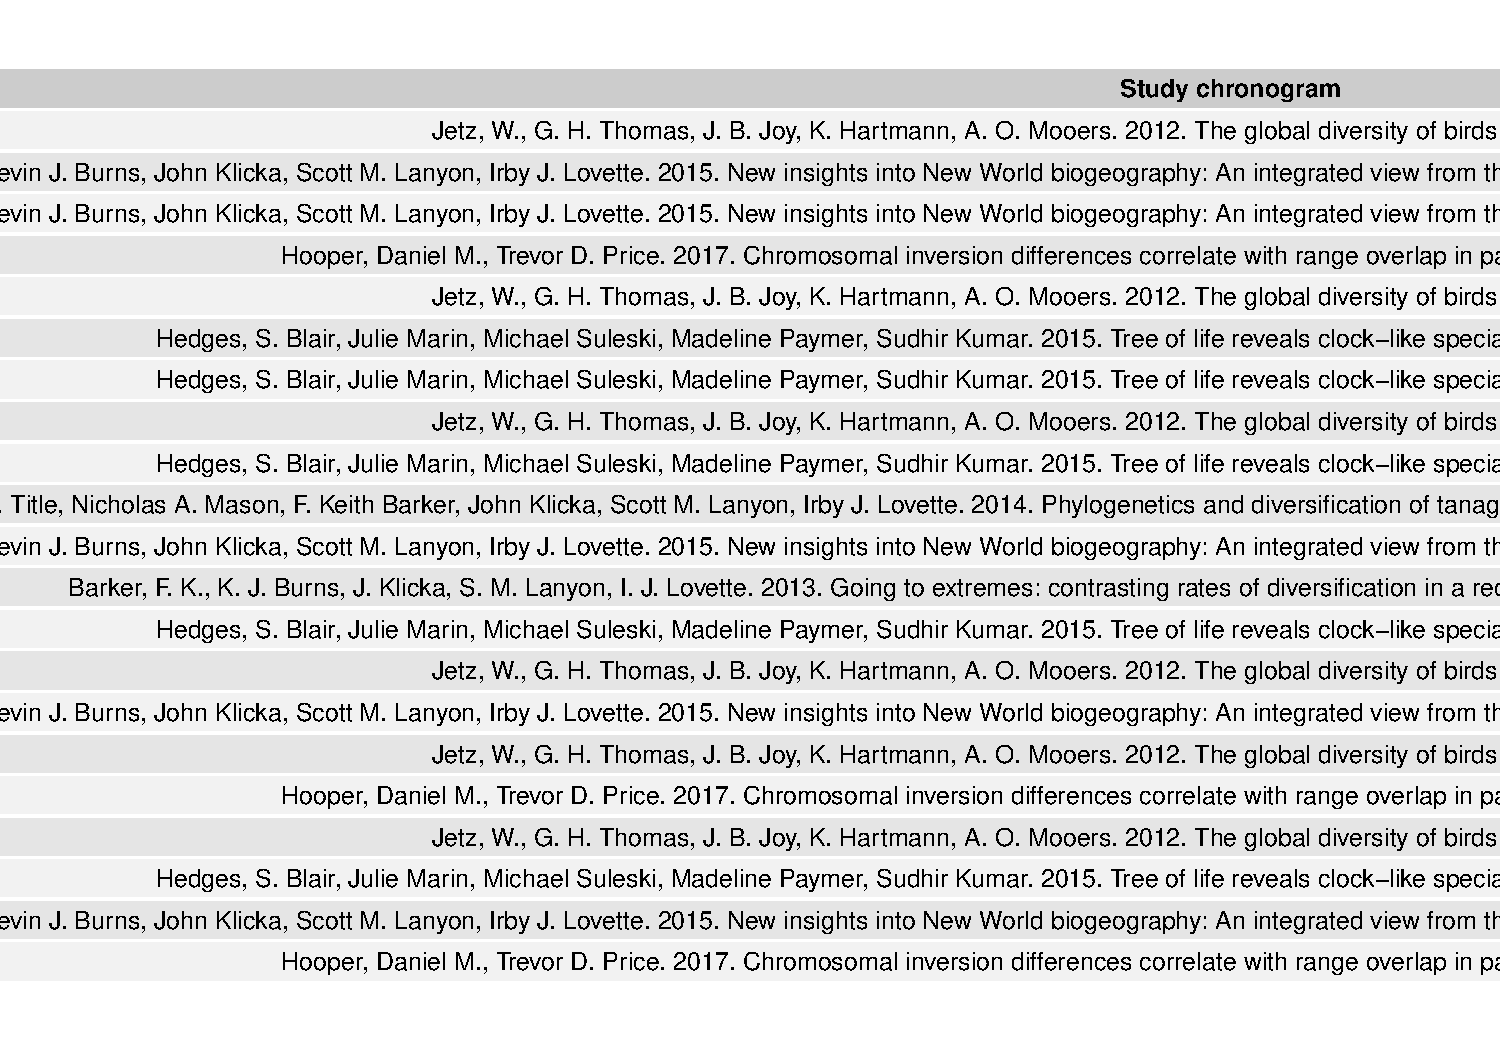
\includegraphics[width=\linewidth]{../tables/table-fringillidae-small-example.pdf}
\end{table}


%%%%%%%%%%%%%%%%%%%%%%%%%%%%%%%%%%%%%%%%%%%%%%%%%%%%%%%%%%%%%%%%%%
%%%%%%%%%%%%%%%%%%%%%%%%    TABLE 2     %%%%%%%%%%%%%%%%%%%%%%%%%%
%%%%%%%%%%%%%%%%%%%%%%%%%%%%%%%%%%%%%%%%%%%%%%%%%%%%%%%%%%%%%%%%%%
\begin{table}
  \caption{Summary of congruified nodes ages, corresponding to step C3 from Figure3}
  \label{tbl:table2}
  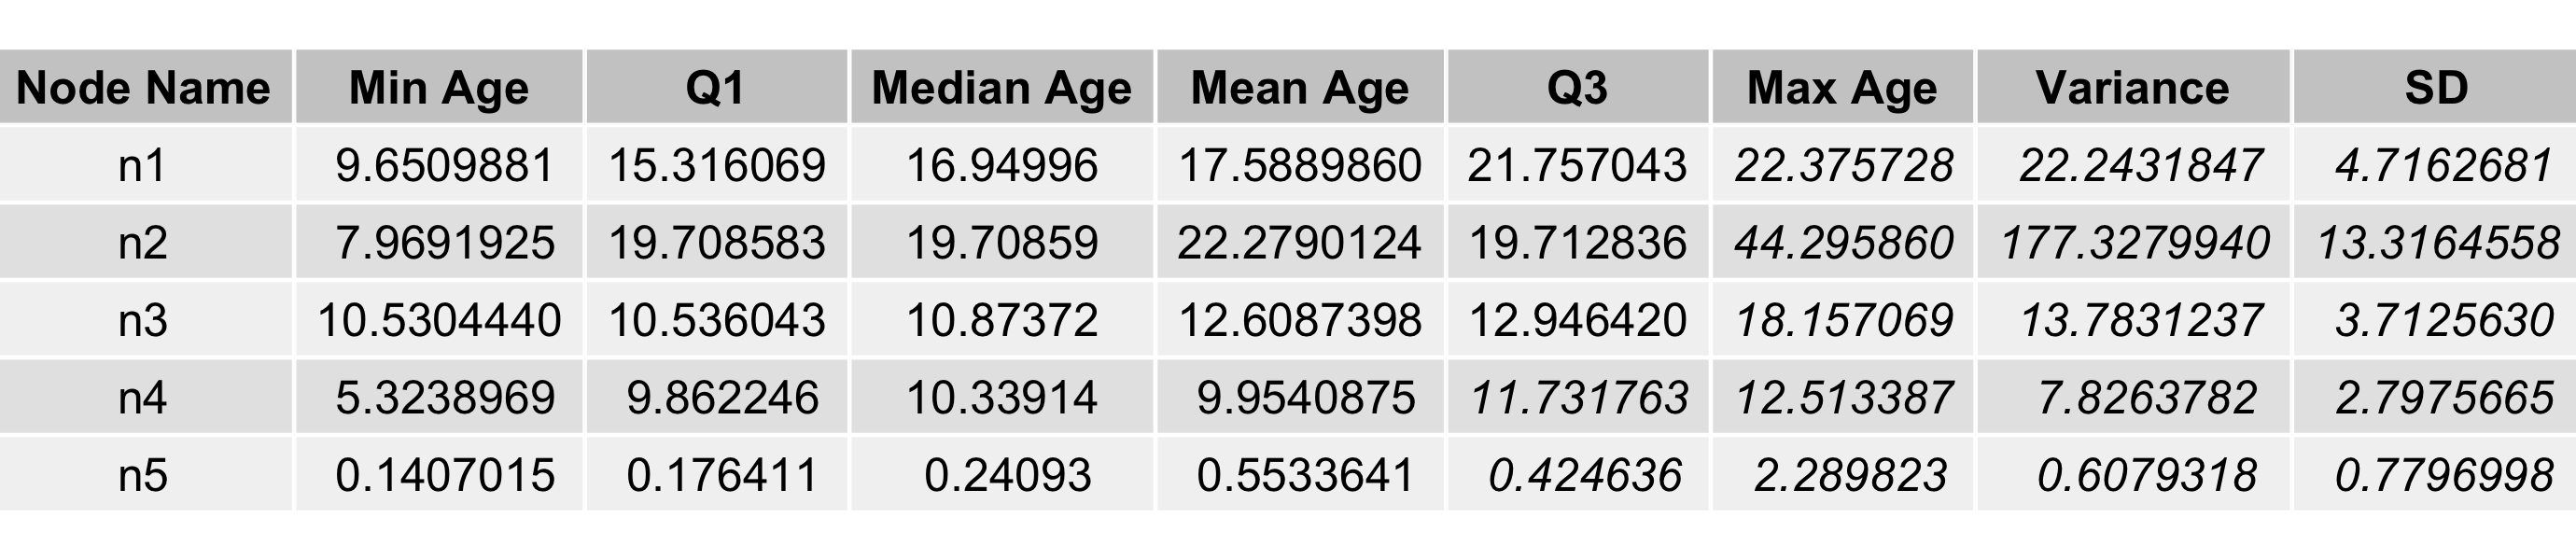
\includegraphics[width=\linewidth]{../tables/table-fringillidae-small-example-summary.png}
\end{table}
